\documentclass[a4paper,12pt]{article} 
\usepackage[T2A]{fontenc}			
\usepackage[utf8]{inputenc}			
\usepackage[english,russian]{babel}	
\usepackage{amsmath,amsfonts,amssymb,amsthm,mathtools} 
\usepackage[colorlinks, linkcolor = blue]{hyperref}
\usepackage{upgreek}\usepackage[left=2cm,right=2cm,top=2cm,bottom=3cm,bindingoffset=0cm]{geometry}
\usepackage{multirow}
\usepackage{graphicx,wrapfig,lipsum}
\usepackage{xcolor}
\usepackage{pgfplots}

\begin{document}

\title{
3.1.3.

Измерение магнитного поля Земли.
\author{Семёнов Андрей Б02-010}
}
\date{29 сентября 2021г.}

\maketitle

\newpage

\textbf{Цель работы:} Измерение магнитного поля Земли.

		
\textbf{В работе используются:} Неодимовые магниты; тонкая нить для изготовления крутильного маятника; медная проволока; электронные весы; секундомер; измеритель магнитной индукции; штангенциркуль; брусок, линейка и штатив из немагнитных материалов; набор гирь и разновесов. 

\section{Теоретические сведения:}
\subsection*{Свойства точечного магнитного диполя}
Простейший магнитный диполь может быть образован витком с током или постоянным магнитом. По определению, магнитный момент $\overrightarrow{P_m}$ тонкого витка площадью $S$ с током $I$ равен
$$
\overrightarrow{P_m}=\dfrac{I}{c}\vec{S}=\dfrac{I}{c}S\vec{n},
$$
где $\vec{S}=S\vec{n}$ есть вектор площади круга контура. Если размеры контура с током или магнитной стрелки малы по сравнению расстоянием до диполя, то соответствующий магнитный диполь называют элементарным или точечным.\\
Магнитное поле точечного диполя определяется по формуле, аналогичной формуле для поля элементарного электрического диполя:
$$
\vec{B}=\dfrac{3(\overrightarrow{P_m},\vec{r})\vec{r}}{r^5} - \dfrac{\overrightarrow{P_m}}{r^3}
$$ 
Во внешнем магнитном поле с индукцией $B$ на точечный магнитный диполь  действует механический момент сил:
$$
\vec{M} = \overrightarrow{P_m}\times \vec{B}.
$$
При этом потенциальная энергия, которой обладает диполь с постоянным $P_m$, равна:
$$
U_{pot} = -(\overrightarrow{P_m},\vec{B})
$$
Когда диполь ориентирован вдоль внешнего поля ($\vec{P_m}\parallel \vec{B}$), он находится в состоянии равновесия ($\vec{M} = 0$). При этом устойчивым будет только состояние, в котором диполь сонаправлен с полем $\vec{P_m}\upuparrows\vec{B}$, поскольку его потенциальная энергия достигает минимума ($U_{min} = -\vec{P_m}B$). При противоположной ориентации энергия будет иметь максимум ($U_{max} = \vec{P_m}B$), и состояние равновесия будет неустойчивым.
\\
В неоднородном внешнем поле на точечный магнитный диполь, кроме момента сил, действует ещё и сила:
$$
\vec{F}= -\vec{\triangledown}\vec{U_{pot}} = (\overrightarrow{P_m},\vec{\triangledown})\vec{B}
$$
Используя формулы для момента силы, силы и энергии, не сложно выяснить, как ведёт себя свободный магнитный диполь в неоднородном магнитном поле: он выстраивается вдоль силовых линий магнитного поля и, кроме того, под действием результирующей силы, возникающей из-за неоднородности поля, втягивается в область более сильного магнитного поля, т.е. в область, где он обладает меньшей энергией.\\
Зная магнитные моменты $P_1 = P_2 = P_m$ двух небольших постоянных магнитов, можно рассчитать силу
их взаимодействия:
$$
F = P_m \dfrac{\partial B}{\partial r}=-6\dfrac{P_m^2}{r^4}.
$$
Полный магнитный момент $\overrightarrow{P_m}$
постоянного магнита определяется намагниченностью $\overrightarrow{p_m}$
вещества, из которого он изготовлен. По определению, намагниченность – это магнитный момент единицы объёма. Для однородно намагниченного шара намагниченность равна:
$$
\overrightarrow{p_m}=\dfrac{\overrightarrow{P_m}}{V}.
$$
Намагниченность — важная характеристика вещества постоянных магнитов, определяющая, в
частности, величину остаточной магнитной индукции $B_r = 4\pi p_m$. Индукция магнитного поля $\overrightarrow{B_p}$
на полюсах однородно намагниченного шара связана с величиной намагниченности и остаточной магнитной индукцией формулами
$$
\overrightarrow{B_p}=\dfrac{8\pi}{3}\overrightarrow{p_m}=\dfrac{2}{3}\overrightarrow{B_r}.
$$
\section*{Описание работы}
\subsection*{Определение магнитного момента магнитных шариков}
\paragraph*{Метод А}
Величину магнитного момента одинаковых шариков можно рассчитать, зная их массу $m$ и определив максимальное расстояние $r_{max}$, на котором они ещё удерживают друг друга в поле тяжести. При максимальном расстоянии сила тяжести шариков равна силе их магнитного притяжения:
\begin{center}
$\dfrac{6P_m^2}{r_{max}^4}=mg\Rightarrow$ \fbox{$P_m = \sqrt{\dfrac{mgr_{max}^4}{6}}$}
\end{center}
\paragraph*{Метод Б}
Если сила сцепления двух одинаковых шаров диаметром $2R$ c магнитными моментами $P_m$ равна:
$$
F_0 = \dfrac{6P_m^2}{(2R)^4} = \frac{3P_m^2}{8R^4}
$$
то минимальный вес цепочки, при которой она оторвётся от верхнего шарика равен: $F = F_{0}(1 + \frac{1}{2^4} + \frac{1}{3^4} + \frac{1}{4^4} + ...) \approx 1.08 F_0$. Тогда\\
\begin{center}
$P_m = \sqrt{\dfrac{8FR^4}{3\cdot1.08}}$
\end{center}
\subsection*{Определение величины магнитного поля Земли}
\paragraph*{Измерение горизонтальной составляющей индукции магнитного поля Земли}
\begin{wrapfigure}{R}{3.5cm}
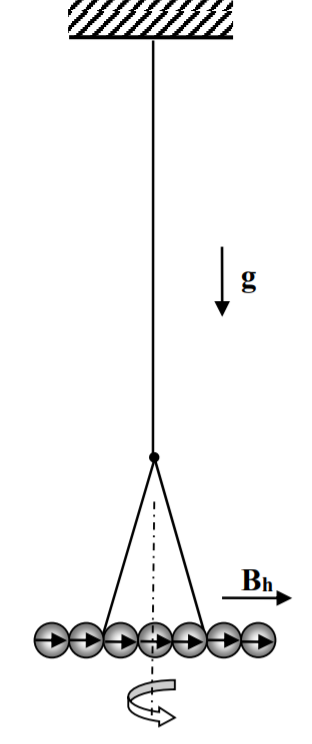
\includegraphics[scale=0.1]{1.png}
\vspace{-60pt}
\end{wrapfigure}  
Магнитная <<стрелка>> образована из $n$ сцепленных друг с другом противоположными полюсами шариков и с помощью $\Lambda$-образного подвеса подвешена в горизонтальном положении. При отклонении «стрелки» на угол $\theta$ от равновесного положения в горизонтальной плоскости возникают крутильные колебания вокруг вертикальной оси, проходящей через середину стрелки. При малых амплитудах уравнение колебаний
стрелки имеет вид:
$$
I_n \dfrac{d^2 \theta}{dt^2} + P_0 B_h \theta = 0,
$$ 
где $P_n = nP_m$ -- полный магнитный момент магнитной <<стрелки>>, $B_h$ -- горизонтальная составляющая магнитного поля Земли, $I_n \approx \dfrac{1}{3}n^3 m R^2$, тогда период колебаний $T_n = kn$, где $k = 2\pi \sqrt{\dfrac{mR^2}{3P_m B_h}}$. Измеряя зависимость $T=T(n)$, найдём $B_h$:
\begin{center}
$B_h = \dfrac{4\pi^2 m R^2}{3k^2P_m}$
\end{center}
\begin{wrapfigure}{R}{6cm}
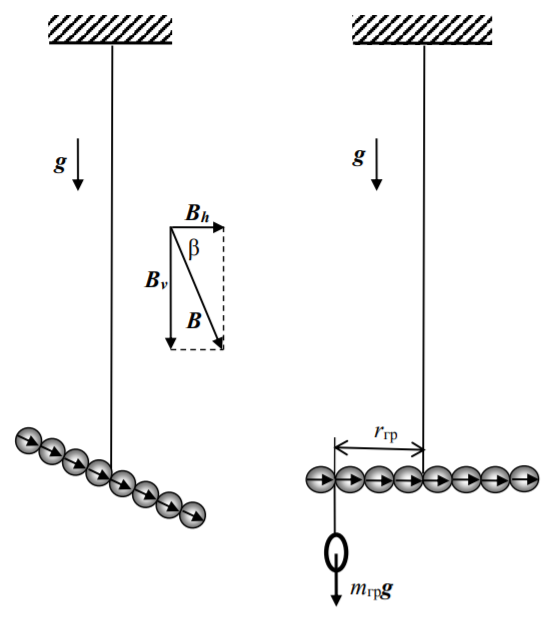
\includegraphics[scale=0.5]{2.png}
\end{wrapfigure} 
\paragraph*{Измерение вертикальной составляющей индукции магнитного поля Земли. Магнитное наклонение.}
Магнитная «стрелка», составленная из чётного числа шариков и подвешенная на тонкой нити за середину, расположится не горизонтально, а под некоторым, отличным от нуля, углом к горизонту. Это связано с тем, что вектор $\vec{B}$ индукции магнитного поля Земли в общем случае не горизонтален, а образует с горизонтом угол $\beta$, зависящим от географической широты $\varphi$
места, где проводится опыт. Величина угла $\beta$
называется магнитным наклонением.\\
С помощью небольшого дополнительного грузика «стрелку» можно «выровнять». Момент $M$ силы тяжести уравновешивающего груза пропорционален числу $n$ шариков, образующих магнитную «стрелку» $M(n) = m_{cargo}gr_{cargo} = n P_m B_v$, пусть $M(n) = bn$
Тогда:
\begin{center}
$B_v = \dfrac{b}{P_m}$
\end{center}
\section*{Ход работы}
\begin{enumerate}
\item Определим параметры шариков: масса 12 штук $m_{12} = 10.007\pm 0.001~\text{г}$, тогда масса одного $m = (8.339 \pm 0.001)*10^{-1}~\text{г}$, диаметр $d = 5.64 \pm 0.01~\text{мм}$.\\
Для измерения $r_max$ поместим шарики по разные стороны деревянной линейки так, чтобы они всё ещё притягивались, и будем подкладывать листы бумаги между ними до тех пора, пока сила тяжести не пересилит силу притяжения. Измеренный $r_{max} = 1.58 \pm 0.05~\text{см}$. Тогда:
\begin{center}
$P_m = 29.2 \pm 0.3~\text{эрг/Гс}, p_m = 310 \pm 11~\text{Гс}, B_r = 3896 \pm 140~\text{Гс},  B_p = 2.59 \pm 0.09~\text{кГс}$
\end{center}
\item Потом собираем установку для измерения горизонтальной составляющей магнитного поля Земли. Перед непосредственным измерение проверим, можно ли пренебречь упругостью нити при измерении периода колебаний. Для этого сделаем из шариков кольцо, чтобы магнитный момент был нулевым (близким к нулю), и посмотрим на его период колебаний. 
Далее измерим зависимость $T(n)$:
\begin{table}[h]
\centering
\begin{tabular}{|l|l|l|l|l|l|l|l|l|l|l|}
\hline
$n$ & 12    & 11    & 10    & 9     & 8     & 7     & 6     & 5     & 4     & 3    \\ \hline
$T$, с & 2.9 & 2.76 & 2.48 & 2.38 & 1.84 & 1.72 & 1.56 & 1.3 & 1.04 & 0.76 \\ \hline
\end{tabular}
\end{table}
\begin{center}
\begin{tikzpicture}[scale=1]
    	\begin{axis}[
    		axis lines = left,
        	xlabel = {$n$, th},
        	ylabel = {$T$, s},
        	ylabel style={green, scale=1},
        	xlabel style={green, scale=1},
        	%xmin=0, xmax=9,
        	title={Зависимость $T(n)$},
        	legend style={at={(0.03,-0.4)},anchor=west}
    		]
    		\addplot +[green, only marks]  plot[
			error bars/.cd,
			x dir = both,
			x fixed relative = 0.01,
			y dir = both,
			y fixed relative=0.01,
		    ]
		    table[x=n, y=T, col sep=semicolon]{Plot1.txt};
		    \addplot[color=red, domain=0:12]{0.2378 * x + 0.077509};
    	\end{axis}
    \end{tikzpicture}
\end{center}
Полученный коэффциент наклона $k= 0.237 \pm 0.002~\text{с}$. Следовательно:
\begin{center}
\textbf{$B_h = 0.532 \pm 0.006~\text{Гс}$}
\end{center}
\item Для магнитных <<стрелок>> вычислим $M(n)$:

\begin{minipage}{0.4\textwidth}
\begin{tabular}{|l|l|l|}
\hline
n  & $m_{cargo}$, г  & M, дин см \\ \hline
12 & 0.222 & 508.432         \\ \hline
10 & 0.086 & 142.892        \\ \hline
8  & 0.222 & 314.585       \\ \hline
6  & 0.222 & 193.847        \\ \hline
4  & 0.222 & 120.738        \\ \hline
\end{tabular}
\end{minipage}
\begin{minipage}{0.6\textwidth}
\begin{tikzpicture}[scale=1]
    	\begin{axis}[
    		axis lines = left,
        	xlabel = {$n$, th},
        	ylabel = {$M$, dyne cm},
        	ylabel style={green, scale=1},
        	xlabel style={green, scale=1},
        	%xmin=0, xmax=9,
        	title={Зависимость $M(n)$},
        	legend style={at={(0.03,-0.4)},anchor=west}
    		]
    		\addplot +[green, only marks]  plot[
			error bars/.cd,
			x dir = both,
			x fixed relative = 0.01,
			y dir = both,
			y fixed relative=0.01,
		    ]
		    table[x=n, y=M, col sep=semicolon]{Plot2.txt};
		    \addplot[color=red, domain=0:10]{48.46 * x + 121.8};
    	\end{axis}
    \end{tikzpicture}
\end{minipage}
Полученный коэффциент наклона $b = 48 \pm 2~\text{дин}\cdot\text{см}$. Тогда
\begin{center}
\textbf{$B_v = 1.66 \pm 0.04~\text{Гс}$}
\end{center} 
\item Индукция магинтного поля Земли $B = \sqrt{B_v^2 + B_h^2} = 1.74 \pm 0.05~\text{Гс}$. Это фиаско. Нужно $0.60 - 0.65$ Гс.
А магнитное наклонение $\beta= \text{arctg}~\dfrac{B_v}{B_h} = \text{arctg}~\dfrac{1.66}{0.532} = 72^\circ\pm 10^\circ$.
\item Расчитаем по методу Б.
\begin{center}
$P_m = \sqrt{\dfrac{8FR^4}{3\cdot1.08}}$
\end{center}
Получим $P_m = 21.9 \text{эрг/Гс}$, следовательно: $p_m = 233 \text{Гс}, B_r = 2930 \text{Гс},  B_p = 1.96 \text{кГс}$
\end{enumerate}
\section{Выводы:}

\newpage
\end{document}